\only<article>{
  \chapter{Fairness.}
}
\label{ch:fairness}
\only<article>{ When machine learning algorithms are applied at scale,
  it can be difficult to imagine what their effects might be. In this
  part of the book, we consider notions of fairness as seen through
  the prism of conditional independence and meritocracy. The first
  notion requires that we look deeper into directed graphical models.
  
  The problem of fairness in machine learning and
  artificial intelligence has only recently been widely
  recognised. When any algorithm is implemented at scale, no matter
  the original objective and whether it is satisfied, it has
  significant societal effects. In particular, even when considering
  the narrow objective of the algorithm, even if it improves it
  overall, it may increase inequality.
  
  In this course we will look at two aspects of fairness. The first
  has to do with disadvantaged populations that form distinct social
  classes due to a shared income stratum, race or gender. The second
  has to do with meritocratic notions of fairness.

  This chapter requires some knowledge of decision theory (See
  Appendix~\ref{ch:decision-problems}) to understand the principles of
  expected utility maximisation and graphical models (See
  Appendix~\ref{ch:graphical-models}) to understand the idea of conditional independence.
}

\section{Introduction.}


\only<article>{ Fairness is a concept that has received much attention
  recently when applied to large-scale algorithmic decision
  making. However, the very concept of fairness is not well-defined
  and encompasses many different ideas. Some of those relate to fair
  treatment of individuals: \emph{Meritocracy} is the idea that people
  should receive rewards according to their merit. \emph{Equal
    treatment} is the related notion that similar people should be
  treated similarly under similar circumstances. Some concepts are
  related more to the treatment of different groups:
  \emph{Proportional representation} is the idea that proportions of
  different groups in society should be reflected in every facet of
  society. Finally \emph{non-discrimination} captures the notion of
  not treating people differently depending on sensitive
  characteristics.  }

\only<presentation>{
  \begin{frame}
    \frametitle{Fairness}
    What is it?
    \begin{itemize}
    \item<2-> \alert{Meritocracy}.
    \item<3-> Proportionality and representation.
    \item<4-> Equal treatment.
    \item<5-> \alert{Non-discrimination}.
    \end{itemize}
  \end{frame}
}

\begin{frame}
  \frametitle{Meritocracy}
  \only<article>{

    Meritocracy embodies the principle that merit should be
    rewarded. A common example are admissions to universities. Some
    type of summary, typically a grade obtained from high school, is
    used to represent the underlying merit of individuals.
  }
  \uncover<2->{
    \begin{example}[College admissions]
      \only<article>{ In this example, we have two students. In terms
        of grades, student $B$ is clearly better. If we can only
        accept one of them, and given no other information, it seems
        like the natural choice is student $B$.  }
      \begin{itemize}
      \item Student $A$ has a grade 4/5 from Gota Highschool.
      \item Student $B$ has a grade 5/5 from Vasa Highschool.
      \end{itemize}
    \end{example}
  }
  \only<article>{Grades, by themselves, are typically insufficient information. It might be that grades from some high-schools are inflated and do not represent the quality of individuals accurately. So, let us suppose we now consider the information.}
  \uncover<3->{
    \begin{example}[Additional information]
      \only<article>{
        In particular, let us suppose that we have statistics on how well students from different high school do, depending on their high school grade.
      }
      \begin{itemize}
      \item 70\% of admitted Gota graduates with 4+ get their degree.
      \item 50\% of admitted Vasa graduates with 5 get their degree.
      \end{itemize}
      \only<article>{
        All other thing being equal, it is now more likely that student $A$ will graduate. So perhaps we should take in $A$ and not $B$.
      }
    \end{example}
  }

  \uncover<4->{We still don't know how a \alert{specific} student will
    do!}
  \only<article>{ Since these are only statistics, they not
    necessarily predictive of an individual student's ability.
    Ideally, we would like to admit the students that we expect to do
    well, given the information that we have. However, this
    information is typically not enough for us to make reliable
    predictions.  In addition, we might want to also make sure that
    everybody has a chance to obtain a good education. In order to
    achieve this, we might want to promote ethnic or gender equality
    through university admissions.  Unfortunately, there is no ideal
    solution and we must always balance the benefit of individual
    students with that of specific societal groups as well as society
    as a whole.  }
  

\end{frame}


\only<presentation>{
  \begin{frame}
    \frametitle{Hiring decisions}
    \begin{columns}
      \begin{column}{0.5\textwidth}
        \includegraphics[height=\textheight]{../figures/cmu-headcount}
      \end{column}
      \begin{column}{0.5\textwidth}
        \includegraphics[width=\columnwidth]{../figures/amazon-hiring}
        \\
        \includegraphics[width=\columnwidth]{../figures/recruitement-automation}
      \end{column}
    \end{columns}
  \end{frame}


  \begin{frame}
    \frametitle{Group fairness and proportionality}
    \includegraphics[width=\textwidth]{../figures/genomics-diversity}
    \url{https://qz.com/1367177/}
  \end{frame}

}

\begin{frame}
  \frametitle{Solutions}
  \only<article>{These solution methods are not completely exclusive, and can be implemented simultaneously to some extent.}
  \begin{itemize}
  \item<1-> Admit \alert{everybody}? \only<article>{This suggests that everybody is admitted to at least one university, perhaps even their university of choice. However, it requires that there is enough teaching capacity for all students in the first year. Subsequently, we expect the students who were not qualified to drop out. Of course, this is unfair to the qualified students, as it drains resources that could have been used for them.}
  \item<2-> Admit \alert{randomly}? \only<article>{Completely random decisions are not considered fair, because they do not take into account any information. However, randomisation can also be used in conjunction with grades to ensure that everybody has a shot.}
  \item<3-> Use \alert{prediction} of individual academic performance? \only<article>{The more information we have, the better we can predict academic performance. A grade from high school is one indicator, but more data can be used to obtain better predictions. Of course, no prediction is perfect.}
  \item<4-> Should we take into account \alert{group membership} or other population information? \only<article>{For many reasons, students in some groups can perform differently in standardised tests, even though their innate talents may be no different than students not in the group. The classical example of this is high school teachers discouraging girls from mathematics.}
  \end{itemize}
  
\end{frame}


\only<article>{
  \begin{example}[Hiring decisions.]
    As a further example, consider gender balance in hiring decisions.
    Typically, received applications are screened, so that some
    applicants undergo through an interview process. At the end, some
    of the interviewed applicants will be hired. There are two
    decision points here, with most people being cut off at the first
    point: the screening. To automate this process, Amazon worked on
    a resume-screening program.~\footnote{\url{https://www.reuters.com/article/us-amazon-com-jobs-automation-insight-idUSKCN1MK08G}}
    However, this was scrapped after it was discovered that it
    predominantly favoured men. The reason is not entirely clear, but
    it was probably due to the fact that they trained the system on
    their own screening decisions, and given that the tech industry
    predominantly hires men in the first place, women were likely
    rejected in the screening phase. 
  \end{example}
}


\section{Group fairness.}
\only<article>{ Let us now take a look at concepts of fairness related
  to \emph{group membership}. This includes concepts such as equal
  treatment, equality of opportunity and generally lack of
  discrimination.  The general idea is that we would like for members
  of society to follow trajectories through life that do not strongly
  depend on their membership in sensitive groups. For example, gender
  should not play a role in academic achievement. Ethnic heritage
  should have no influence on annual income. Unfortunately, the
  underlying societal dynamics create situations where group
  membership becomes important.

  In this section, and throughout this chapter, we will imagine that
  an individual is interacting with a system, which makes decisions
  about the individual, such as whether or not to give them a
  loan. These result in a certain outcome, such as the individual
  using the borrowed money to invest in a business and then having a
  particular annual income. Crucially, these outcomes can be
  correlated with group membership, because of societal dynamics. The
  system designer should make sure that not only the system does what
  it intends, such as giving loans to people that are expected to
  repay them, but also that it does not create inequalities between
  different groups. As we will see later, depending on our fairness
  definition, and on the societal dynamics, this is almost never easy.
  
}

\begin{frame}
  \frametitle{Bail decisions}

  \only<article>{ For a more detailed example, let us consider bail
    decisions in the US court system. When a defendant is charged, the
    judge has the option to either place them in jail pending trial,
    or set them free, under the condition that the defendant pays some
    amount of 'bail', or guarantee. The amount of bail (if any) is set to deter
    flight or a relapse, and is returned to the defendant after the
    trial.

    This process sometimes includes the use of a software tool called
    \texttt{COMPAS}, which gives risk scores for the possibility of
    flight, recidivism or violent behaviour. These scores are taken
    into account by judges when making decisions.  In some cases, it
    appears as though automating this procedure might lead to better
    outcomes. But is that generally true?
  }


  \only<presentation>{
    \begin{columns}
      \begin{column}{0.5\textwidth}
        \centering
        \begin{tikzpicture}
          \node at (0,0) (judge) {\includegraphics[width=0.3\columnwidth]{../figures/judge}};
          \uncover<2->{
            \node at (-2,-2) (jail) {\includegraphics[width=0.3\columnwidth]{../figures/jail}};
            \draw[->] (judge) -- (jail);
          }
          \uncover<3->{
            \node at (2,-2) (bail) {\includegraphics[width=0.3\columnwidth]{../figures/bail}};
            \draw[->] (judge) -- (bail);
          }

          \uncover<4->{
            \node at (-2,-4) (trial) {\includegraphics[width=0.3\columnwidth]{../figures/trial}};
            \draw[->] (jail) -- (trial);
          }
          \uncover<5->{
            \draw[->] (bail) -- (trial);
          }
          \uncover<6->{
            \node at (2,-4) (arrest) {\includegraphics[width=0.3\columnwidth]{../figures/handcuffs}};
            \draw[->] (bail) -- (arrest);
          }
        \end{tikzpicture}
      \end{column}
      \begin{column}{0.5\textwidth}
        \centering
        \uncover<7->{
          \includegraphics[width=\textwidth]{../figures/judge-fairness}
        }
      \end{column}
    \end{columns}
  }

  \only<article>{In this setting, a defendant $t$ appears before a
    judge with observable features $x_t \in \CX$, and a sensitive group
    variable $z_t \in \CZ$. The judge employs a specific policy $\pol$ to
    select a decision $a_t \in \CA$, with
    \begin{equation}
      \pol(a_t \mid x_t, z_t)
    \end{equation}
    denoting the probability of action $a_t$ given the individual's features, as well as the sensitive variable. We can assume that the policy is fixed ahead of time, and thereafter decisions are made according to the policy.
    After the judge makes their decision, they observe an outcome $y_t$ sampled from some potentially unknown distribution with parameter $\theta$:
    \begin{equation}
      P_\theta(y_t \mid x_t, z_t), \qquad      P_\theta(y_t \mid x_t, z_t, a_t), 
    \end{equation}
    denoting the probability of $y_t$ given the individual's features
    and the action taken. Here, there are two possibilities. Either
    the outcome $y_t$ depends only on the observed features, or the
    action as well. The correct formulation depends on the meaning of
    the action.

    \paragraph{Actions that affect the outcome.}
    Let us first consider a simple set of actions $\CA = \{0, 1\}$,
    where a defendant is granted $(a_t = 1)$ or denied $(a_t = 0)$
    bail.  If a defendant is not given bail, they must remain in jail,
    and will always be at the trial $(y_t = 0)$. This costs both the
    government and the defendant, so the judge prefers not to deny
    bail too often.  On the other hand, if the defendant is granted
    bail, there is a chance they will re-offend, or will fail to
    attend trial $(y_t = 1)$. Consequently, we can define the
    following utility function\footnote{See
      Appendix~\ref{ch:decision-problems}} for the judge, that roughly
    reflects those preferences:
    \begin{equation}
      U(a, y) = a - y.
    \end{equation}
    While this weighs the judge's two main concerns equally, we can also imagine different formulations: e.g. if the judge thinks it is much more important to keep people out of jail than to prevent re-offences until trial, they might select a function such as : $U(a, y) = 10a - y$.


    \paragraph{Actions that do not affect the outcome.} In this
    scenario, the only way for the actions to not affect the outcome
    is if everybody is released, with the judge's action only being a
    confidential note on the case file. Then their action cannot
    affect the outcome, since it is only revealed to the judge. The
    utility function can be based on the accuracy of predictions, so
    we can simply set it to $U(a,y) = a - y$.
    
    \paragraph{The optimisation problem.} Now, given the parameter $\param$ of the unknown distribution, the judge can find a decision rule $\pol$ maximising utility in expectation
    \begin{equation}
      \label{eq:expected-utility-judge}
      \E_\param^\pol(U) = \sum_{x,z} P_\theta(x, z) \sum_a \pol(a | x, z) \sum_y P_\theta(y | a, x, z) U(a,y).
    \end{equation}
    In practice, of course, $\param$ is not known but we have some training data $D = (x_t, z_t, a_t, y_t)_{t=1}^T$, collected with some historical policy $\pol_0$, and  we have to resort to one of the following solutions. Firstly, estimating some $\hat{\param}$ from the data and replacing that in the expectation. Secondly, calculating a posterior distribution $\beta(\param | D)$ and maximising $\int_\Param \E_\param^\pol(U) \dd \bel(\param | D)$. Thirdly, maximising an unbiased estimate of expected utility, as shown below:
    \begin{align*}
      \E^\pol_\param(U)
      &=
        \sum_{x,z} P_\theta(x, z) \sum_a \pol(a | x, z) \sum_y P_\theta(y | a, x, z) U(a,y) \\
      &\approx
        \frac{1}{T} \sum_{t} \sum_a \pol(a | x_t, z_t) \sum_y P_\theta(y | a, x_t, z_t) U(a,y)
        \approx
        \frac{1}{T} \sum_{t} \frac{\pol(a_t | x_t, z_t)}{\pol_0(a_t | x_t, z_t)} U(a_t,y_t).
    \end{align*}
    The first approximation simply replaces the feature distribution with its empirical approximation.
    The second approximation is a bit more delicate, and is a type of importance sampling,\index{importance sampling} as explained in more detail in Section~\ref{sec:monte-carlo}.
    This is because, in the original data we have only some specific $a_t, y_t$ for every individual $t$, where $a_t$ was selected by some historical policy $\pol_0$. For that reason, we must use importance sampling in order to estimate the utility of any policy $\pol$. Unfortunately, the policy $\pol_0$ is also unknown and must be estimated from the data. So, we are left with deciding between modelling $P_\param(y | a, x, z)$ or $\pol_0(a | x, z)$.

    However, doing so may have unintended effects, as treatment of different groups may be unequal. For that reason, we may have to add explicit fairness constraints to our optimisation problem. 

  }
\end{frame}  

\begin{frame}
  \frametitle{Demographic parity and equality of opportunity.}

  \only<article>{Let us take a look at how many individuals are given
    different scores. Figure~\ref{fig:risk-bias} shows the proportions
    of individuals obtaining different risk scores as a function of
    their ethnic group. While the general population, and Caucasians
    in particular, have a distribution sharply concentrated in low
    scores, Black defendants obtain much higher risk scores: they are
    almost as likely to be ranked a 10 as the are to be scored a 1. }
  \begin{figure}[H]
    \centering
    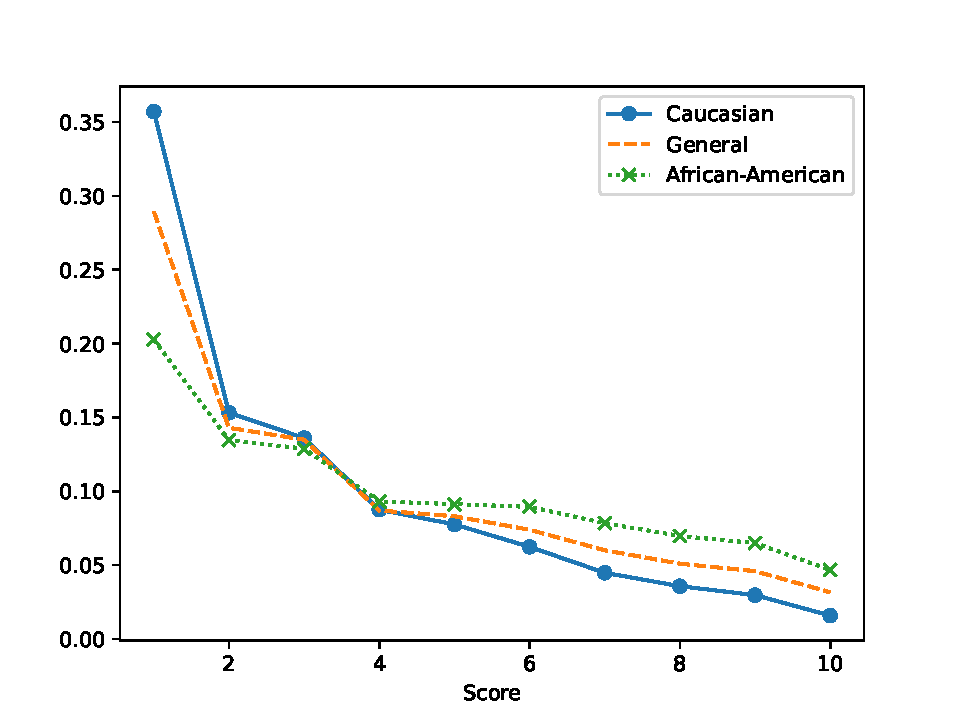
\includegraphics[width=\fwidth]{../figures/Scores-by-race}      
    \label{fig:risk-bias}
    \caption{Apparent bias in risk scores towards black versus white defendants.}
  \end{figure}
  \only<article>{ Typically, we would like to demographic parity
    across groups, either with respect to the decisions, or with
    respect to the outcomes.  Decision parity is called \emph{equality
      of opportunity} and satisfies the following condition
  }
  \begin{equation}
    \label{eq:equality-opportunity}
    \Pr_\param^\pol(a_t | z_t) =       \Pr_\param^\pol(a_t ).
  \end{equation}
  \only<article>{
    In other words, the action (risk score, in this case) is
    independent of the group.  As we see in
    Figure~\ref{fig:risk-bias}, these distributions are quite
    different.  The curve for ``General'' corresponds to
    $\Pr_\param^\pol(a_t )$, while the other two curves correspond to
    $\Pr_\param^\pol(a_t | z_t)$ for $z_t$ being Caucasian and
    African-American respectively.
    
    \emph{Demographic parity} instead relates to outcomes. If this
    condition is satisfied, then the probability distribution of
    outcomes is independent of group membership.
    \begin{equation}
      \label{eq:eqality-outcomes}
      \Pr_\param^\pol(y_t | z_t) =       \Pr_\param^\pol(y_t ).
    \end{equation}

  }
\end{frame}

\begin{frame}
  \frametitle{Calibration.}
  
  \only<article>{On the
    other hand, the scores generated by the software seemed to be very
    predictive on whether or not defendants would re-offend,
    independently of their race. Figure~\ref{fig:imrs} shows that, if
    an individual obtains a high score then they are very likely to
    re-offend, and conversely, they are unlikely to re-offend when
    they have a low score. }
  \begin{figure}[H]
    \centering
    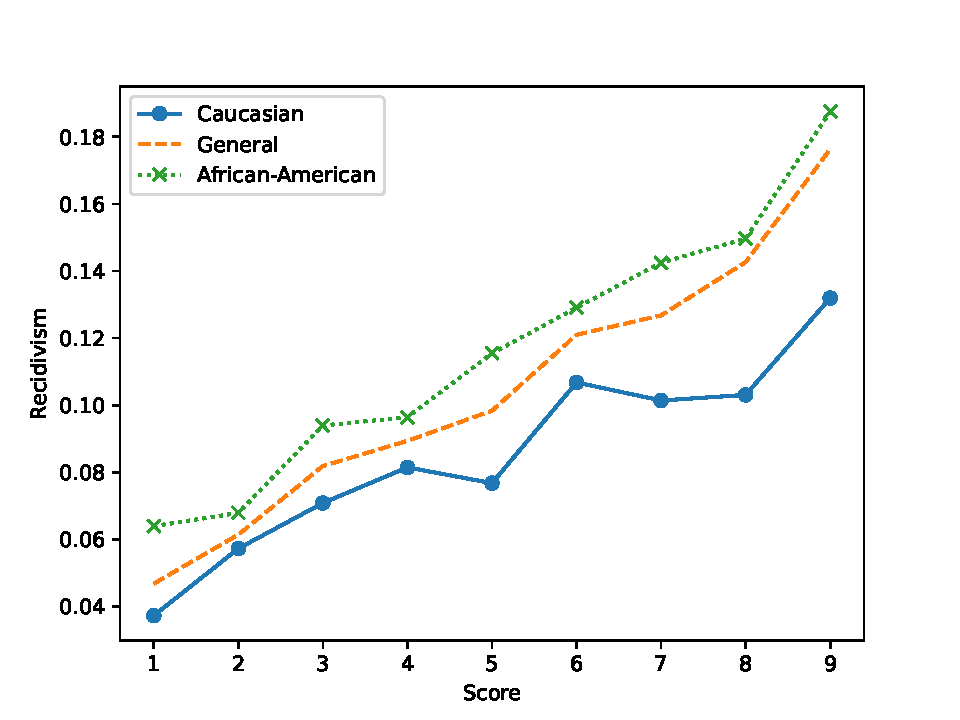
\includegraphics[width=\fwidth]{../figures/calibration-compas}
    \caption{Recidivism rates by risk score.}
    \label{fig:imrs}
  \end{figure}
  \only<article>{
    This concept can be quantified in terms of the conditional distribution of outcomes given the score:}
  \begin{equation}
    \Pr_\param^\pol(y_t | a_t, z_t) =       \Pr_\param^\pol(y_t | a_t).
    \label{eq:calibration}
  \end{equation}
  \only<article>{
    This means that $y_t$ is conditionally independent of $z_t$ given
    the score $a_t$. So, in some sense, the score is sufficient for us
    to predict the outcome, and knowing the race does not help us
    predict any better.
  }
\end{frame}

\begin{frame}
  \frametitle{Balance}
  \only<article>{While the system's predictions seem to be calibrated against the chance of recidivism, this does not mean that race plays no role. Figure~\ref{fig:imrs-risk} breaks down the population in people that re-offended and those that did. For each sub-population, we then plot the proportion of people receiving different scores by race. While people generally have a small probability of obtaining a high risk score, we see that Black defendants obtain much higher scores.}
  
  \begin{figure}[H]
    \centering
    \begin{subfigure}{0.45\textwidth}
      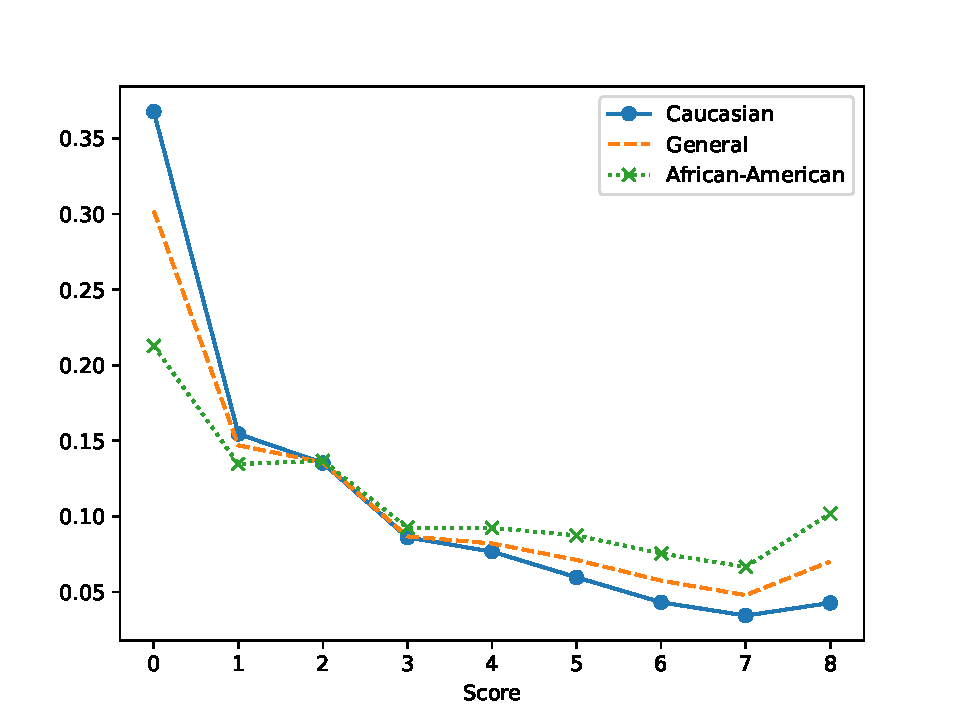
\includegraphics[width=0.95\textwidth]{../figures/balance-non-recidivism-compas}
      \caption{No recidivism}
    \end{subfigure}
    \begin{subfigure}{0.45\textwidth}
      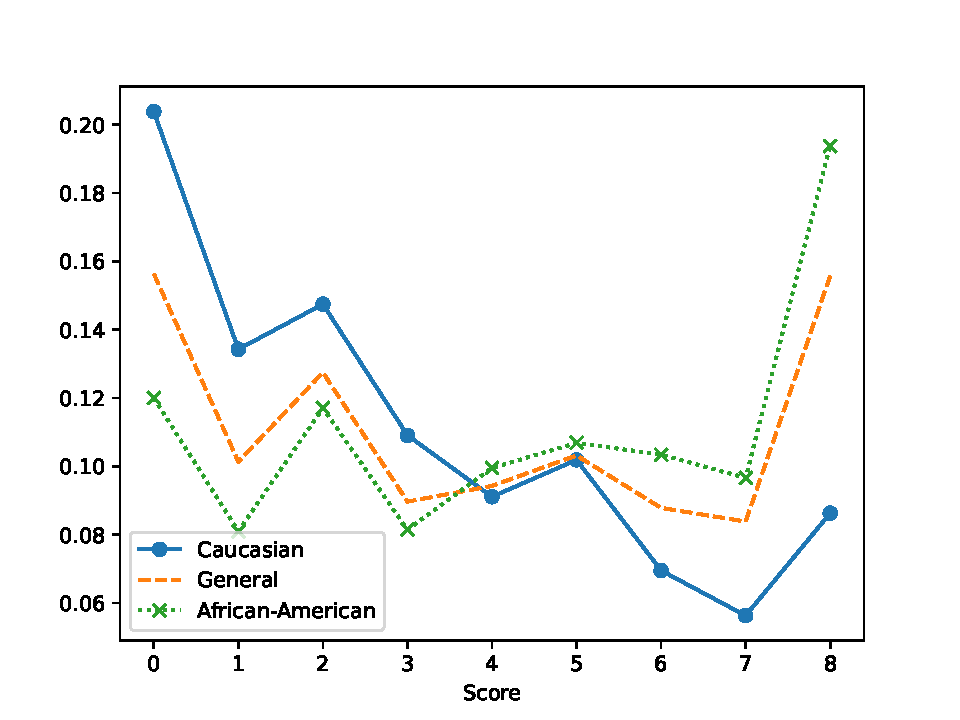
\includegraphics[width=0.95\textwidth]{../figures/balance-recidivism-compas}
      \caption{Recidivism}
    \end{subfigure}
    \caption{Score breakdown based on recidivism rates.}
    \label{fig:imrs-risk}
  \end{figure}
  \only<article>{
    Balance can also be interpreted as a probabilistic condition, of the following form:
  }
  \begin{equation}
    \Pr_\param^\pol(a_t | y_t, z_t) =       \Pr_\param^\pol(a_t | y_t).
    \label{eq:balance}
  \end{equation}
  \only<article>{
    Here we have that $a_t$ is conditionally independent of $z_t$
    given the outcome $y_t$. So, if we partition the population
    according to their outcome, we should find that given the outcome,
    the distribution of scores is the same no matter what their
    race. However, this is not what the example shows: there is a
    strong dependence on race.  }
  
\end{frame}

\only<presentation>{

  \begin{frame}
    \frametitle{Graphical models and independence}
    \begin{itemize}
    \item<1-> Why is it not possible to be fair in all respects?
    \item<2-> Different notions of \alert{conditional independence}.
    \item<3-> Can only be satisfied rarely simultaneously.
    \end{itemize}
    \pause
    \begin{center}
      \begin{tikzpicture}
        \node<5->[RV, hidden] at (-1,1) (p) {$\param$};
        \node<6->[select] at (4,0) (pol) {$\pol$};
        \node<7->[RV] at (0,0) (x) {$x_t$};
        \node<8->[RV] at (2,0) (a) {$a_t$};
        \node<9->[RV] at (1,1) (y) {$y_t$};
        \node<10->[utility] at (3,1) (u) {$\util$};
        \draw<8->[->] (x)--(a);
        \draw<9->[->] (x)--(y);
        \draw<9->[->] (a)--(y);
        \draw<7->[->] (p) to (x);
        \draw<9->[->] (p)--(y);
        \draw<8->[->] (pol)--(a);
        \draw<10->[->] (a)--(u);
        \draw<10->[->] (y)--(u);
      \end{tikzpicture}
    \end{center}
    \begin{itemize}
    \item<5-> $\param$: environment parameters (\alert{latent} variable)
    \item<6-> $\pol$: policy of the decision maker (\alert{decision} variable)
    \item<7-> $x_t$: observation
    \item<8-> $a_t$: action taken
    \item<9-> $y_t$: outcome
    \item<10-> $\util$: \alert{utility}
    \end{itemize}
  \end{frame}
}

\only<article>{ How can we explain this discrepancy? We can show that
  in fact, each one of these different measures of bias in our
  decision rules can be seen as a notion of conditional
  independence. Had $z_t$ been an independent variable, i.e. so that
  $P_\param(x,z) = P_\param(x) P_\param(z)$ and
  $P_\param(y | x,a,z) = P_\param(y | x,a)$, then it would have no
  role. Unfortunately, though, it does influence the distributions of
  the other variables.  }

\begin{frame}

  \begin{example}[Classification]
    \only<presentation>{
      \begin{itemize}
      \item $y$: labels
      \item $a$: label prediction
      \item $U(a, y) = \ind{a = y}$.
      \item Here the outcome is independent of the action:
      \end{itemize}
    }
    \only<article>{
      One setting where the above discussion applies directly are classification problems. There, the outcomes $y$ are simply labels. the decision space $\CA$ is to just predicting a label, and the utility function is the classification accuracy, so that $U(a, y) = \ind{a = y}$. In this setting, $y$ does not directly depend on $a$, since $a$ is just a prediction of the latent label.  More precisely, $y \indep a \mid x$. This allows us to write
    }
    \[
      \Pr_\param^\pol(y_t \mid a_t, x_t, z_t) =   \Pr_\param^\pol(y_t \mid x_t, z_t).
    \]

    \only<article>{
      For binary classification problems in particular, we may be only
      interested in slightly narrower concepts, such as equal false
      negative---$\Pr(a_t = 0 | y_t = 1, z_t = z)$---or false
      positive---$\Pr(a_t = 1 | y_t = 0, z_t = z)$---rates between groups
      $z$.
    }
  \end{example}
\end{frame}
\begin{frame}

  \begin{example}[Regression]
    \only<article>{
      We can also apply these ideas to regression problems. We are again
      asked to simply predict a latent variable $y$. For concreteness,
      assume $y \in \Reals$. Then, the decision space $\CA = \Reals$ as
      well. A standard utility function is the negative squared prediction
      error, so that $U(a, y) = - (a - y)^2$.
    }
    
    In this setting we can also relax our framework to work with
    expectations instead of probabilities. For example, calibration and balance can be written as the conditions:
    \[
      \E_\param^\pol(y_t | a_t, z_t) = \E_\param^\pol(y_t | a_t),
      \qquad
      \E_\param^\pol(a_t | y_t, z_t) = \E_\param^\pol(a_t | y_t),
    \]
    respectively.
    \only<article>{
      This is a useful definition in particular when our
      action is the assignment of a numerical score, as in the COMPAS
      recidivism example. However, this definition is weaker, as the
      expectations of two random variables can be equal when their
      distributions are different.
    }
  \end{example}
\end{frame}
\subsection{Measuring group fairness.}

\only<article>{
  The above discussion focused on the setting where we have a precise
  model parameter $\param$ and policy $\pol$. However, we frequently do
  not know at least one of those things. For example, when we only have
  some observational data generated by some historical policy $\pol$,
  need to estimate $\Pr_\theta^\pol$ somehow. Moreover, these conditions
  will not be perfectly satisfied. How can we measure the deviation from
  these conditions?
}

\only<presentation>{
  \begin{frame}
    \centering
    {\Huge Measuring and optimising fairness and utility.}
  \end{frame}
}
\begin{frame}
  \frametitle{Expected utility.}
  Let us write out expected utility, with $\Pr_\param^\pol(\cdot) \equiv \Pr(\cdot \mid \param, \pol)$
  \[
    \E_\param^\pol(U) = \sum_{x,z,y} \Pr_\param^\pol(y,a,x,z) U(a,y).
  \]
  The $y_t, a_t, x_t, z_t$ is already sampled from $\Pr_\param^\pol$, so we can approximate the expected utility of the \alert{historical policy} with
  \[
    \widehat{E}_n(U) = \sum_{t=1}^n U(a_t,y_t), \qquad a_t, y_t \sim \Pr_\param^\pol.
  \]
  \only<article>{
    Thus, estimating the expected utility of a particular policy is only possible, if we can sample actions and outcomes from $\Pr_\param^\pol$. Of course, this requires having some specific model for sampling outcomes for any given action, as the policy in historical data might have taken different actions from the ones we are taking.
  }
  
  \only<presentation>{
    \begin{block}{Model specification}
      For simplicity, assume $z = x_{1}$, i.e. one of the features.  Then
      \[
        \Pr_\param^\pol(y,a,x,z)
        =
        \underbrace{\Pr_\param(y \mid a, x)}_{\textrm{outcome distribution}}
        \underbrace{\pol(a \mid x)}_{\textrm{policy}}
        \underbrace{\Pr_\param(x)}_{\textrm{feature distribution}}
      \]
    \end{block}
    Using the model, we can estimate the expected utility of any policy.
  }
\end{frame}

\begin{frame}
  \frametitle{Deviation from balance.}
  \only<article>{
    How about measuring whether balance is satisfied?  Unfortunately
    none of these fairness conditions will be satisfied in practice. So
    what are we going to do? A simple idea is to simply look at how far
    away the distribution is from independence. In particular, let us
    look at the difference between those distributions
  }

  \[
    \Pr_\param^\pol(a | y, z), \qquad  \Pr_\param^\pol(a | y).
  \]
  for all values of $y, z$. Let us first look at the total variation distance:
  \[
    \|\Pr_\param^\pol(a | y, z) -   \Pr_\param^\pol(a | y)\|_1
    =
    \sum_a |\Pr_\param^\pol(a| y, z) -   \Pr_\param^\pol(a | y)|_1.
  \]
  \only<article>{
    We can then sum over all possible values of $y, z$ to obtain a
    single measure of how much we deviate from balance. To obtain an
    empirical estimate, we can simply sum over all observations to
    obtain the empirical models:
  }
  \[
    \hat{P}_n(a | y, z) = \sum_t \frac{\ind{a_t = a \wedge y_t = y \wedge z_t = i}}{\ind{y_t = y \wedge z_t = i}}
  \]
  We can then plug those into our original measure:
  \[
    \|\Pr_\param^\pol(a | y, z) -   \Pr_\param^\pol(a | y)\|_1
    \approx
    \sum_a |\hat{P}_n (a| y, z) -   \hat{P}_n(a| y)|.
  \]
  \only<article>{  
    However, we can
    use something else as well, such as the KL divergence:
    \[
      D(\Pr_\param^\pol(a | y, z)  \|   \Pr_\param^\pol(a | y))
      =
      \sum_a \ln \frac{\Pr_\param^\pol(a | y, z)}{\Pr_\param^\pol(a | y)} \Pr_\param^\pol(a | y, z)
    \]
  }
\end{frame}
\subsection{Trading off  utility and fairness.}
\label{sec:trad-util-fairn}
\only<article>{ We have now selected a notion of utility and of
  fairness. We have also seen how to measure utility and fairness in
  practice. How can we choose a policy $\pol$ that optimises for both? The
  general idea is to formalise the problem in terms of a constrained
  or unconstrained optimisation. }
\begin{frame}
  \frametitle{Formalisation of the problem}

  \only<article>{ Let us use $F(\pol, \param)$ for the measure of
    deviation from fairness and $U(\pol, \param)$ for utility. Since
    these two objectives might be conflicting, we need a way to select
    a policy that trades off one with the other.

    We can deal with the problem in two ways. The first is to
    formulate a combined objective that mixes the utility and fairness
    objectives. Then we can formalise the problem as an unconstrained
    optimisation. The second is to optimise one objective and place
    constrains on the other. For example, we can place a limit on how
    much unfairness we are willing to tolerate and maximise
    utility. Or, we can place a limit on how far away we want to be
    from the solution that optimises for utility only, and optimises
    for fairness. Which method to use is application-dependent, but
    also has some computational impact.  }

  \begin{block}{Unconstrained optimisation.}
    \only<article>{The simnplest idea is to treat the utility and fairness symetrically. Then we can simply optimise for their mixture.}
    Let $\lambda \in [0,1]$:
    \[
      \max_\pol (1 - \lambda) U(\pol, \param) - \lambda F(\pol, \param)
    \]
  \end{block}
  \only<article>{
    In this setting, we have an unconstrained optimisation problem. These are typically easier to solve, and we can use simple gradient methods. In particular, note that the gradient with respect to the policy of the unconstrained objective is
    \[
      \nabla_\pol [(1 - \lambda) U(\pol, \param) - \lambda F(\pol, \param)]
      =
      (1 - \lambda) \nabla_\pol U(\pol, \param) - \lambda \nabla_\pol F(\pol, \param).
    \]
    Consqeuently, we only need to move in the direction of the sum of
    these gradients.  The only problem with this formulation is that
    setting the $\lambda$ parameter is not very intuitive, in
    particular if one of the two quantities is more sensitive to the
    policy than the other.  }

  

  \only<article>{Let us now look at two different ways of modelling the problem as constrained optimisation. This might be useful if we need to have guarantees on fairness or utility. In the first formulation, we maximise utility and constrain the fairness deviation. In the second, we minimise the fairness deviation and constrain the utility.}
  \begin{block}{Constrained fairness.}
    \only<article>{In this setting, we have an upper bound $\epsilon$ on the amount of fairness deviation we can allow.     Let $\epsilon \geq 0$:}
    \begin{align*}
      \max_{\pol \in \Pol} U(\pol, \param)\\
      \textrm{s.t.} F(\pol, \param) \leq \epsilon.
    \end{align*}
  \end{block}

  \only<article>{Since the best we can do for fairness deviation is to have $F(\pol, \param) = 0$, it makes sense to upper bound it by an amount $\epsilon$. Let us now look at the converse problem, maximising fairness, while making sure that the utility is not much worse than the best we can get. }
  \begin{block}{Constrained utility.}
    \only<article>{In this setting, we want to limit the amount of sub-optimality $\epsilon$ we have relative to the optimal policy that ignores fairness.}
    Let $\epsilon \geq 0$:
    \begin{align*}
      \max_{\pol \in \Pol} F(\pol, \param)\\
      \textrm{s.t.} U(\pol, \param) \geq  \max_{\pol' \in \Pol} U(\pol', \param) - \epsilon
    \end{align*}
  \end{block}
  \only<article>{Here it's important to measure the loss in performance relative to the utility-maximising policy. To understand this, consider the case where $U : \Pol, \Param \to [0,1]$. Then we could have chosen the constrained $U(\pol, \param) \geq 1 - \epsilon$, i.e. that our policy is at least $\epsilon$-close to the highest possible utility. However, it might be impossible to find a policy with this value: indeed, it could be that $\max_{\pol'} U(\pol', \param) < 1 - \epsilon$, in which case we would never find a policy satisfying the constraint. For that reason, we specify the constraint in terms of the performance difference relative to the highest \emph{attenable} utility.}
\end{frame}

\only<article>{
  \subsection{Dealing with unknown parameters $\param$.}

  The above discussion assumed that we know what the underlying
  parameter $\theta$ is. However, in practice this is never the case: We
  only have some observational data $D = (x_t, z_t, a_t, y_t)_{t=1}^T$, which
  indirectly gives us information about $\theta$. There are three
  methods for dealing with this problem. Using a point estimate of the
  parameter, using a Bayes-optimal policy, or finding a policy that
  guarantees utility and fairness with high probability. All approaches require some parametric model family for $\cset{[P_\param(y | a, x, z), P_\param(x, z)]}{\param \in \Param}$. For simplicity, let us consider the unconstrained optimisation of
  \[
    V(\pol, \param) \defn (1 - \lambda) U(\pol, \param) - \lambda F(\pol, \param).
  \]
  Maximising $V(\pol, \param)$ directly is not possible since $\param$ is not known. However, we can formulate the following concrete methods for solving it.
  
  \paragraph{Use an estimated $\hat{\param}$.} The idea here is to replace the unknown $\param$ with an estimated value $\hat{\param}$. Here, for example, we could perform maximum-likelihood inference to find an estimate for $\param$:
  \[
    \hat{\param} \defn \argmax_{\param \in \Param} \prod_{t=1}^T P_\param(y_t | a_t, x_t, z_t) P_\param(x_t, z_t).
  \]
  We then need to solve the following optimisation problem, replacing the unknown value of the parameter with its estimate:
  \[
    \max_{\pol \in \Pol} V(\pol, \hat{\param}).
  \]
  However, this approach completely ignores the uncertainty about $\param$. In practice, this makes a rather large difference, especially in some group fairness settings, where increased uncertainty makes the optimal policy quite different.

  \paragraph{Bayesian decision theory.} The Bayesian solution is simple. Starting with a prior distribution $\bel$ on $\Param$, calculate the posterior $\bel(\param \mid D)$ using the data $D$. We now need to solve the following optimisation problem, which integrates over all possible values of the unknown parameter, weighted by their probability:
  \[
    \max_{\pol \in \Pol} \int_\Param V(\pol, \param) \dd \bel(\param \mid D).
  \]
  For a given policy space $\Pol$ the introduction of an integral does not make things much harder than in the case where $\param$ is known. In fact, if we are using gradient descent to find the optimal policy, we only need to change the algorithm to \emph{stochastic} gradient descent, where the randomness comes from the fact that we sample parameters from the posterior distribution. This is because we can write the gradient as follows:
  \[
    \nabla_\param \int_\Param V(\pol, \param) \dd \bel(\param \mid D)
    =
    \int_\Param \nabla_\param V(\pol, \param) \dd \bel(\param \mid D)
    \approx
    \frac{1}{n} \sum_{i=1}^n \nabla_\param V(\pol, \param^{(i)}), \qquad \param^{(i)} \sim \bel(\param \mid D).
  \]
  In the last step, we are approximating the integral with $n$ samples from the posterior, and taking the gradient separately for each one. This solution was implemented in \cite{dimitrakakis2017:subjective-fairness} and contrasted with a maximum likelihood approach.

  \paragraph{High probability bounds.} It is also worth mentioning that it is typically possible to construct some confidence set $\hat{\Param}$ so that $\Pr(\param \notin \hat{\Param}) \leq \delta$. This means that high probability, we the true parameter lies in $\hat{\Param}$. Then we can instead solve the optimisation problem:
  \[
    \max_{\pol \in \Pol} \min_{\param \in \hat{\Param}} V(\pol, \param),
  \]
  which takes a \emph{pessimistic} view of the uncertainty. That is, for every possible choice of policy, it finds the best-case parameter among the plausible ones. This is not necessary: we could simply choose another parameter in $\hat{\Param}$, but with this methodology, we are quite sure that the actual value of the policy is not going to be worse. The only downside is that the maximin optimisation problem may not be easily solveable. It is also interesting to consider the $\max_{\pol \in \Pol} \max_{\param \in \hat{\Param}} V(\pol, \param)$ optimisation problem instead, which gives an \emph{optimistic} solution. This can turn out to be advantageous when we will actively collect data using our policy.
}

\section{Individual fairness}
\only<presentation>{
  \begin{frame}
    \centering
    {\Huge Individual fairness}
  \end{frame}
}
\only<article>{ An altogether different type of fairness concept is
  individual fairness. This is linked to the notion of meritocracy, i.e.
  that ``better'' people should have ``better'' outcomes. But what do
  we mean by better? This depends strongly on the context: people that
  are better than others in one respect might be worse in another,
  i.e. student A might be better in Math than student B, but worse in
  History, and student A might prefer the Math department to the
  History department and vice-versa.  In addition, what is better for
  a person is a direct result of that person's preference.  An
  alternative concept for individual fairness is treating similar
  people similarly. Then the question is, what do we mean by similar?
  Again, in some contexts different features of individuals might be
  more important as a way to measure similarity: when considering
  university applicants, their grades are probably more important to
  determine which student should be accepted to a degree program,
  rather than their eye colour.

  A lot of the variables we might be interested in are not
  observed. For example, we might want to know the true potential and
  skill of a student in Math. However, the only thing we have is their
  exam or high-school grades, which are mere proxys for their true
  skills. While one of the easiest ways to deal with meritocracy is to
  define worth precisely respect to those observed variables, it is a
  good idea to use inferred measures of worth if possible. However,
  this requires building some type of model.

  Finally, even though we are making decisions about individuals,
  frequently these are made about multiple individuals at once. This
  is is the case in university placements, for example, where
  thousands of students submit their preferences for different
  university programmes, and then they are placed depending on their
  own preferences, as well as their grades. Thus, the problem faced by
  the decision maker is not a simple classification, but rather a
  matching problem.
}

\begin{frame}
  \begin{block}{Main variables for individual fairness.}
    \only<article>{To define fairness with respect to a decision maker, we need to specify what is observed by the decision maker, and what the decision maker performs.}
    \begin{itemize}
    \item $x_i \in \Reals^d$: Individual features. \only<article>{That's what we observe about the $i$-th individual. In the university setting this would correspond to their grades and other personal information.}
    \item $w_i \in \Reals$: Individual worth. \only<article>{This can be taken to mean how well the individual is expected to perform in university, e.g. their expected grade. However, this quantity is not directly observed.}
    \item $u_i : \CA \to \Reals$: Individual utility. \only<article>{This is how much the individual gains by the decision. For simplicity, we can imagine that $i$ is only impacted by the decision regarding them, rather than anybody else, so we can just define a function $u_i(a_i)$ instead.}
    \item $a \in \CA$: Action taken by the decision maker. \only<article>{For
        example, $a$ could specify which applicants are admitted to
        university, with $a_i$ specifying the university to which 
        applicant $i$ is admitted.}
    \item $\pol$: The decision maker's policy for making decisions.
      \only<article>{This is defined as $\pol(a | x)$, the probability of a decision given the features of the population. In some settings, the policy makes decisions for each individual separately. Then we can define their policy $\pol(a_i | x_i)$ in terms of individual decisions $a_i$ and observations $x_i$. This also means that the decision about any one individual does not depend on either the features of or the decisions for other individuals:
        \[
          \pol(a | x) = \prod_i \pol(a_i | x_i). 
        \]
        However, in many cases, such as in university admissions, we make our decisions about everybody at the same time. Then the above independence condition does not hold, and the decision maker's choice depends on everybody's observations.}
    \end{itemize}
  \end{block}
\end{frame}

\subsection{Meritocracy.}

\only<article>{Let us first discuss the concept of meritocracy as it
  relates to an individual's inherent worth. The assumption here is
  that individuals can be ranked in terms of their worth, so that
  individuals with more worth are deserving of higher rewards. Of
  course, this idea is only easy to work with when we know the worth
  of each individual, as well as how much each one values possible
  rewards.

  In addition, we have to have a notion of the worth of rewards. The
  simplest assumption is that for any pair of possible rewards
  (e.g. university placements), everybody prefers one of them to the
  other. However, we do not expect everybody to have the same
  preferences. Indeed, in university placements, each student
  typically submits and ordered list of preferences and they are
  matched to programs according to their preferences and their
  grades.

  In the definition below, we assume that every individual has a
  specific, invariant, inereht worth. They also have a clear
  preference over the decision maker's actions.
}


\begin{frame}
  \frametitle{Meritocracy for given utilities and worths.}
  \only<article>{ The following definitions are applicable for any
    type of decision making over individuals. An important point is
    that there is a distinction between decisions being fair and
    policies being fair. Requiring that individual decisions satisfy a
    fairness constraint is much stricter than a similar requirement
    for policis. }
  \begin{definition}
    A \textbf{decision} $a$ is \textbf{fair} if, for all $i,j$, we have $w_i > w_j \Rightarrow u_i(a) \geq u_j(a)$.
  \end{definition}
  \only<article>{In the above definition, a person with a higher worth than another is guaranteed to obtain at least as good an outcome as another person of lower worth. If we think about a single decision affecting multiple individuals, then such a fairness property is hard to satisfy: in some cases there may not exist any such fair decision, as shown in the example below.}
  \begin{example}
    \begin{tabular}{c||c|c|c}
      $w$ &  &  $a = 0 $ & $a = 1$\\
      \hline
      1  & $u_1$ & 0 & 1\\
      0  & $u_2$ & 1 & 0
    \end{tabular}
  \end{example}
\end{frame}
\begin{frame}
  \begin{definition}
    A \textbf{policy} $\pol$ is \textbf{fair} if, for all $i,j$ it holds that: $\E_\pol [u_i | w] > \E[u_j | w] \Rightarrow w_i > w_j$.
  \end{definition}
  
  \only<article>{ Let us consider problems where the decision maker
    has a binary choice, e.g. to accept or reject a loan
    application. In particular, the decision rule may be restricted so
    that the decision has to depend only on a \emph{score}, e.g. the
    credit score. Let $w_i$ be the score of the $i$-th
    individual. Typically, the decision $a_i$ about an individual $i$
    does not depend on the decision about any other individual. Hence,
    the decision rule can be factorised as
    $\pol(a | w) = \prod_i \pol(a_i | w_i)$. This is typically the
    case when individuals appear sequentially, and we must make a
    decision for each one of them in turn, as long as the decision
    rule $\pol$ remains fixed.
    
    However, in some cases $\pol$ itself depends on a population of individuals. This is the case in cohort selection, when we need to select some individuals from a set.
  }


  \begin{example}[Ranking and top-$k$ cohort selection.]
    \only<article>{
      In this setting, we assume we have a set of $n$
      individuals, with the $i$-th individual receiving an evaluation
      $w_i$. We need to choose individuals from the set so that
      $a_i = 1$ if we select an individual, and $0$ otherwise. We can
      assume that all individuals prefer being selected.  The
      selection algorithm $\pol$ creates an allocation
      $a=(a_1, \ldots, a_n)$. A simple way to perform the allocation
      to first rank the individuals so that $w_{i} > w_{i+1}$. We then
      can assign $a_i=1$ for all $i \leq k$.
    }
    \only<presentation>{
      \begin{itemize}
      \item $n$ individuals
      \item $i$-th individual receiving an evaluation
        $w_i$.
      \item $a_i = 1$ if we select an individual, and $0$ otherwise.
      \item Ranked selection algorithm $\pol$: first rank the individuals so that $w_{i} > w_{i+1}$. We then     can assign $a_i=1$ for all $i \leq k$.
      \end{itemize}
    }
  \end{example}
\end{frame}
\only<article>{
  This, however, creates a problem. What if the $k$-th individual has value $w_k$, but there exist more individuals of equal value, so that e.g. $w_{k+1} = w$? Due to our constraint on only selecting $k$ individuals from the set, we now have a problem: if we select $k$ and not $k+1$, we are treating the individuals differently, even though their characteristics are exactly the same. The simplest way to fix that is to choose between $k$ or $k+1$ with probability $1/2$ each. The same problem occurs when we want to match multiple individuals to one of many possible allocations, as is done in university entrance. The obvious solution there is also randomisation. Even though some people find randomisation fundamentally unfair, it is the only method offering equitable treatment (though not equitable outcomes) for indistinguishable individuals.
}

\begin{frame}
  \begin{example}{Matching problems.}
    \only<article>{ In classical matching problems, such as university
      admissions, each individual $i \in \{1, \ldots, n\}$ have an
      individual evaluation $w_i$, calculated according to some
      uniform criteria, calculated from individual features $x_i$,
      such as test results, age, etc. Each individual $i$ also
      generates a preference score $u_i$ so that they prefer
      university $k$ to university $l$ if
      $u_i(k) \geq u_i(l)$.\footnote{In practice, it is sufficient to
        give a ranking of universities rather than numerical
        scores. In addition, universities may have inhomogeneous
        preferences, but in this example they simply prefer students
        with the highest score.}  The matching algorithm $\pol$
      creates an allocation $a=(a_1, \ldots, a_n)$ so that $a_i$ is
      the university to which candidate $i$ is matched. The algorithm
      $\pol$ satisfies a \emph{stable matching} condition: this means
      for a candidate $i$ to be preferred for a position at a
      university $k$ to a candidate $j$, either (a) $i$ must prefer
      $k$ more than $j$ (i.e.  $u_i(k) > u_j(k)$) or (b) candidate $i$
      must be preferred by the university to $k$ (i.e. $w_i >
      w_j$). Consequently, it is impossible for both $w_j < w_i$ and
      $u_j(k) < u_i(k)$ to hold and student $j$ to be allocated to
      university $k$.

      In the following, there are three
      individuals $(1,2,3)$ three universities $(x,y,z)$, with the
      preferences:}
    \begin{itemize}
    \item $u_1(x) > u_1(y) > u_1(z)$,
    \item $u_2(z) > u_2(y) > u_2(x)$
    \item $u_3(z) > u_3(x) > u_3(y)$ 
    \end{itemize}
    and $w_1 > w_2 > w_3$. A stable matching is then
    $a_1 = x, a_2 = z, a_3 = y$.

    \only<article>{ For the sake of the argument, assume
      $u_1(x) = u_2(z) = u_3(z)$, so as to make the utilities
      comparable. Then for this allocation $u_1 = u_2 > u_3$.
    }
    
  \end{example}
\end{frame}

\only<article>{In practice, we do not have direct access to an
  individual's worth. However, we may have a model that estimates
  worth based on their individual features. To be as general as
  possible, we can assume a probabilistic model
  $P_\param(w_i | x_i)$ that assigns a distribution over worths
  $w_i$ for individuals with features $x_i$. Then we want our
  decisions to be fair in expectation. This expectation is taken with respect to both the randomness due to our modelling, and the potential randomness due to our decision rule.

  What if two students had almost, but not exactly the same grades, and one was assigned a place, while the other not. Is that fair? Is it perhaps fairer to randomise to some extent, so that, while the best students are guaranteed a place, the ones further down the ranking might still have a chance? After all grades are not the absolute truth: they are but a noisy, biased measurement of an individual's academic capacity. In the section below, we will discuss how decision rules can be made smoother more generally, and not just through randomising over identical individuals.
}


\subsection{Fairness as smoothness.}
\only<article>{ Another principle for individual fairness is
  \emph{treating similar people similarly}. For example, consider a
  company hiring for multiple positions. While there maybe a few
  outstanding candidates who are all hired, a relative of the CEO, who
  is a mediocre candidate, is also hired. The relative stands out
  because he is treated differently to other similar candidates.

  To formalise this principle, we need to first assume that each
  candidates $i$ is describe by some features $x_i \in \CX$, and that
  a metric $d : \CX \times \CX \to \Reals_+$ is defined on $\CX$, so
  that similar individuals will have a smaller distance.

  We also need to define what we mean by similar treatment. For
  simplicity, we will first consider the case where the DM is making
  decisions about each individual separately. Hence, they take
  decision $a_i \in \CA$ for individual $i$ with probability
  $\pol(a_i | x_i)$. Then we need to define some distance or
  divergence $D[\pol(a_i | x_i) | \pol(a_j | x_j)]$ between the
  decision distributions for two different individuals.

  
  Finally, we also need to define what the decision maker wants to
  achieve. This can be captured through a utility function $U$,
  measuring the quality of DM's policy. In the simplest scenario, we
  can assume that the DM has a simple payoff function
  $\rho : \CX \times \CA \to \Reals$, representing their expected payoff
  $\rho(x,a)$ for each possible observe feature and action taken.

  In the case where the policy is making separate decisions for each
  individual, there are two possible problems. The first problem is to make individual decisions
  for a finite given population $\CX = \{x_1, \ldots, x_T\}$. This allows us to define the utility
  in terms of the sum of individual payoffs:
  \[
    U(\pol) \defn \sum_{t=1}^T \sum_{a \in \CA} \rho(x_t, a) \pol(a_t = a | x_t).
  \]
  The second problem is to define a policy that will be applied in a
  \emph{potential} population. This means that we do not have to make a
  decision now, but we will have to fix a policy that will be applied
  later to individuals drawn independently\footnote{This is only a mild assumption on the setting where decisions are made independently for each individual.} from some distribution
  $P$. Then the utility of any policy $\pol$ over some distribution $P$
  can be written as:
  \[
    U(\pol) \defn \int_{\CX} dP(x) \left[\sum_{a \in \CA} \rho(x, a) \pol(a_t = a | x)\right].
  \]
  For simplicity, we can assume that $P$ is known, but it could also have been estimated from data. Similarly, $\rho$ may be an arbitrary evaluation function, or it could be somehow estimated. For example, if we have a model of rewards $r \in \Reals$ for different action and observation combinations $p(r | x, a)$, then we can set the payoff function to be our expected reward $\rho(x, a) \defn \E[r | x,a] = \int_{-\infty}^\infty r p(r | x,a) dr$ for taking action $a$ for individual $x$.
  
  To impose a smoothness constraint on the policy, we require it to be Lipschitz-smooth with respect to the metric on the observed features. Together with the objective of maximising utility, we can define the following constrained maximisation problem:
  \begin{block}{Treating similar individuals similarly.}
    For a given utility $U$, metric $d$ on $\CX$ and divergence $D$:
    \begin{equation}
      \max_\pol  U(\pol), \qquad
      \st  D[\pol(a_i | x_i), \pol(a_j | x_j)] \leq d(x_i,x_j). 
      \label{eq:lipschitz-fairness}
    \end{equation}
  \end{block}
  Of course, in some cases the utility might not be known perfectly, and we can use a Bayesian approach. It is also possible that we have not settled on an appropriate metric $d$ with respect to the features. Finally, the policy may not have the independence property, so the above Lipschitz condition may not be properly defined. There are also differences in the available solutions for the optimisation problem when we are dealing with a fixed population versus a distribution over populations.  We will go through all of these later. 
}
\only<presentation>{
  \begin{frame}
    \begin{block}{Treating similar individuals similarly.}
      \begin{itemize}
      \item $d(x_i,x_j)$: Distance between individuals $i,j$. 
      \item $D[\pol(a_i | x_i), \pol(a_j | x_j)]$: Distance between policy decisions.
      \item Utility function $U(\pol)$.
      \end{itemize}
      Our goal is to find a decision rule $\pol$ maximising  $U(\pol)$, 
      so that it is Lipschitz-smooth with respect to $D, d$:
      \[
        D[\pol(a_i | x_i), \pol(a_j | x_j)] \leq d(x_i,x_j)
      \]
    \end{block}
    \only<article>{When $D(P,Q) = \max_{a \in A} |\log [P(a)/Q(a)]|$ then $\pol$ satisfies differential privacy with $d(x,y) = \epsilon \|x - y\|_1$}.
  \end{frame}
}

\begin{frame}{Connection to meritocracy.}
  Consider a decision maker that is choosing applicants to hire
  $(a = 1)$. For any two applicants with respective features
  $x_i, x_j$, we need to assume that they both prefer being hired to 
  not being hired. On the other hand, the DM prefers to hire
  applicants that result in higher utility. In particular, hiring
  applicant $x$ results in utility $u(x)$. Let us now define the
  utility of a policy, when applied to a single applicant, as
  \[
    \E^\pi (U | x) = \pi(a = 1| x) u(x).
  \]
  Trivially, our policy should be such that we tend to hire people with higher utility to us.
  If the utility function is $L$-Lipschitz, then $|u(x) - u(x')| \leq L d(x,x')$. Now consider the case where $x'$ can get an unfair advantage through nepotism. However, if our policy is smooth, it requires $\pi(a = 1 | x) \geq \pi(a = 1 | x') - d(x,x') \geq \pi(a = 1 | x') - |u(x) - u(x')|/L$. In addition, since our policy must be a maximising policy, if  $u(x) > u(x')$, then $\pi(a = 1 | x) \geq \pi(a=1 | x')$.
\end{frame}

\subsection{Individual decisions for a fixed population.}
\only<article>{
  Let us start with the simplest case, by defining the optimisation problem \eqref{eq:lipschitz-fairness} when we are asked to provide a policy for a finite population $\CX$. Then we need only consider the policy and constraint for all the people in $\CX$. More specifically, for the $i$-th person with data $x_i$ in the dataset $\CX$, the probability of taking action $a$ is $\pol(a \mid x_i)$. How should we parametrise the policy?

  Let us look at the case of a finite number of actions. Then, the simplest method is to simply define a parameter vector $\vparam_t \in \Simplex^{|\CA|}$ for the $t$-th individual, so that
  $\param_{t,a} \defn \pol(a \mid x_t)$. This leads to the optimisation problem
  \[
    \max_{\vparam} \sum_{t=1}^T  \sum_{a \in \CA} \rho(x_t, a) \param_{t,a},
    \qquad \st \sum_{a \in \CA} \param_{t,a} = 1, \param_{t,a} \geq 0 \forall t, a.
  \]
  Here both the objective and the constraints are linear with respect to the parameters, hence the overall problem is a \emph{linear program}.

  Let us look at the smoothness constraints now. If we limit ourselves only to the observed population, there is a finite number of constraints: $D[\pol(a \mid x_i)\|\pol(a \mid x_j)]$ for $i, j \in [T]$. The simplest choice for $D$ is total variation between two distributions:
  \[
    D_{TV}(P\|Q) \defn \max_{A \subset \Omega} |P(A) - Q(A)| = \frac{1}{2} \|P - Q\|_1 = \frac{1}{2} \sum_{\omega \in \Omega} |P(\omega) - Q(\omega)|.
  \]
  This results in the following set of constraints for our problem:
  \[
    \sum_{a \in \CA} |\param_{i,a} - \param_{i,j}| \leq d(x_i, x_j).
  \]
  Since $d(x_i, x_j)$ does not depend on the parameters, the problem remains linear.

  On the other hand, if we want to parametrise differently, e.g. by calculating the probabilities of different actions through a softmax distribution, then the problem becomes non-linear. This is something we must do anyway, in the case where the population is not fixed and so we will describe it in the next section.
}
\subsection{Unknown population policies.}
If we need to fix a policy before seeing the population, then we must use a parametrised policy that can give us a probability distribution over $a$ for any possible $\bx \in \CX$ where $\CX$ is a compact subset of $\Reals^n$.
A simple parametrisation is a linear-softmax network,\footnote{We cannot use a linear network, because then $\pol(a \mid \bx) = \vparam_a^\top x$, and the probabilities of different actions cannot sum to one.}
with $\vparam_a \in \Reals^n$ for all actions $a$, given by:
\[
  \pol(a \mid \bx) = \frac{e^{\vparam_a^\top x}}{\sum_{a' \in \CA} e^{\vparam_{a'}^\top \bx}}.
\]
This is not really difficult to work with, but we have a potential problem when considering the smoothness constraints. If we let $d(\bx, \bx') = \|bx - \bx'\|$ then the Lipschitz condition is in fact a condition on the gradient:
\[
  \nabla_\bx \pol(a \mid \bx) \leq 1, \qquad \forall \bx \in \CX
\]



In particular, we can no longer make it so 
\subsection{Group fairness properties of smooth policies.}
\begin{frame}\frametitle{Smoothness and parity.}
  Can group fairness be satisfied in this setting?
  To define groups, we select $S, T \subset \CX$. We can say a policy satisfies approximate parity between the groups if:
  \begin{definition}{$\epsilon$-parity}
    \[
      \|\pol(a | x \in S) - \pol(a | x \in T)\|_1 \leq \epsilon.
    \]
  \end{definition}
  We can also similarly define the worst-case bias for some action:
  \begin{definition}{Bias for some action $a$:}
    \[
      \max_\pol \pol(a | x \in S) - \pol(a | x \in T)
      \qquad
      \textrm{s.t. $\pol$ is Lipschitz}
    \]
  \end{definition}
  \only<article>{The main problem here is that if we are required to be smooth, but one set has most of its members in one subset.}
\end{frame}

\subsection{Fair ranking.}

\subsection{Fair cohort selection.}

\section{Exercises}

\only<article>{
  \begin{exercise}
    Consider the following problem, where $z$ is Bernoulli(1/2) and $x \Reals^2$ is a normally distributed variable with mean $(0,z)$ and identity covariance matrix. There are two actions and outcomes, with the outcome being $y_t = 1$ with probability $1/(1 + e^{x_a})$.
    [Add more details]
  \end{exercise}
}

%%% Local Variables:
%%% mode: latex
%%% TeX-engine: xetex
%%% TeX-master: "book"
%%% End:
